% Created by tikzDevice version 0.12.3 on 2020-05-27 23:27:08
% !TEX encoding = UTF-8 Unicode
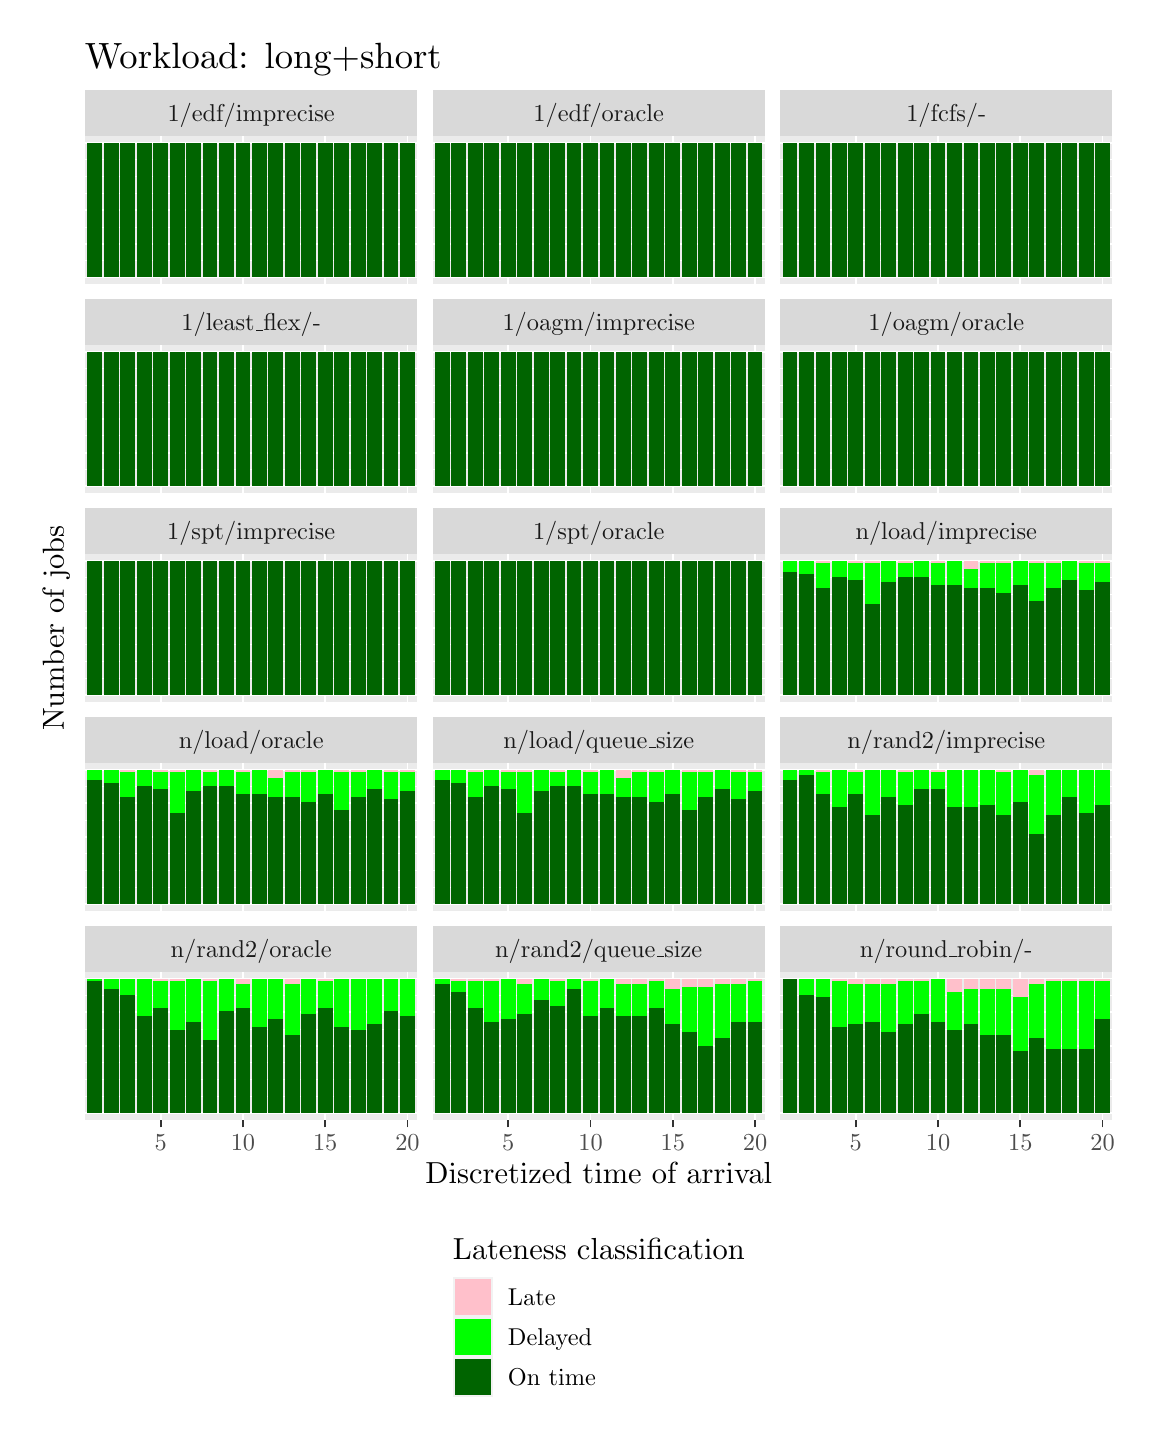
\begin{tikzpicture}[x=1pt,y=1pt]
\definecolor{fillColor}{RGB}{255,255,255}
\path[use as bounding box,fill=fillColor,fill opacity=0.00] (0,0) rectangle (397.48,505.89);
\begin{scope}
\path[clip] (  0.00,  0.00) rectangle (397.48,505.89);
\definecolor{drawColor}{RGB}{255,255,255}
\definecolor{fillColor}{RGB}{255,255,255}

\path[draw=drawColor,line width= 0.6pt,line join=round,line cap=round,fill=fillColor] (  0.00,  0.00) rectangle (397.48,505.89);
\end{scope}
\begin{scope}
\path[clip] ( 20.71,413.24) rectangle (140.80,466.66);
\definecolor{fillColor}{gray}{0.92}

\path[fill=fillColor] ( 20.71,413.24) rectangle (140.80,466.66);
\definecolor{drawColor}{RGB}{255,255,255}

\path[draw=drawColor,line width= 0.3pt,line join=round] ( 20.71,421.74) --
	(140.80,421.74);

\path[draw=drawColor,line width= 0.3pt,line join=round] ( 20.71,433.88) --
	(140.80,433.88);

\path[draw=drawColor,line width= 0.3pt,line join=round] ( 20.71,446.02) --
	(140.80,446.02);

\path[draw=drawColor,line width= 0.3pt,line join=round] ( 20.71,458.16) --
	(140.80,458.16);

\path[draw=drawColor,line width= 0.6pt,line join=round] ( 20.71,415.67) --
	(140.80,415.67);

\path[draw=drawColor,line width= 0.6pt,line join=round] ( 20.71,427.81) --
	(140.80,427.81);

\path[draw=drawColor,line width= 0.6pt,line join=round] ( 20.71,439.95) --
	(140.80,439.95);

\path[draw=drawColor,line width= 0.6pt,line join=round] ( 20.71,452.09) --
	(140.80,452.09);

\path[draw=drawColor,line width= 0.6pt,line join=round] ( 20.71,464.23) --
	(140.80,464.23);

\path[draw=drawColor,line width= 0.6pt,line join=round] ( 48.06,413.24) --
	( 48.06,466.66);

\path[draw=drawColor,line width= 0.6pt,line join=round] ( 77.79,413.24) --
	( 77.79,466.66);

\path[draw=drawColor,line width= 0.6pt,line join=round] (107.51,413.24) --
	(107.51,466.66);

\path[draw=drawColor,line width= 0.6pt,line join=round] (137.24,413.24) --
	(137.24,466.66);
\definecolor{fillColor}{RGB}{0,100,0}

\path[fill=fillColor] ( 21.61,415.67) rectangle ( 26.96,464.23);

\path[fill=fillColor] ( 27.55,415.67) rectangle ( 32.90,464.23);

\path[fill=fillColor] ( 33.50,415.67) rectangle ( 38.85,464.23);

\path[fill=fillColor] ( 39.44,415.67) rectangle ( 44.79,464.23);

\path[fill=fillColor] ( 45.39,415.67) rectangle ( 50.74,464.23);

\path[fill=fillColor] ( 51.33,415.67) rectangle ( 56.68,464.23);

\path[fill=fillColor] ( 57.28,415.67) rectangle ( 62.63,464.23);

\path[fill=fillColor] ( 63.22,415.67) rectangle ( 68.57,464.23);

\path[fill=fillColor] ( 69.17,415.67) rectangle ( 74.52,464.23);

\path[fill=fillColor] ( 75.11,415.67) rectangle ( 80.46,464.23);

\path[fill=fillColor] ( 81.06,415.67) rectangle ( 86.41,464.23);

\path[fill=fillColor] ( 87.00,415.67) rectangle ( 92.35,464.23);

\path[fill=fillColor] ( 92.95,415.67) rectangle ( 98.30,464.23);

\path[fill=fillColor] ( 98.89,415.67) rectangle (104.24,464.23);

\path[fill=fillColor] (104.84,415.67) rectangle (110.19,464.23);

\path[fill=fillColor] (110.78,415.67) rectangle (116.13,464.23);

\path[fill=fillColor] (116.73,415.67) rectangle (122.08,464.23);

\path[fill=fillColor] (122.67,415.67) rectangle (128.02,464.23);

\path[fill=fillColor] (128.62,415.67) rectangle (133.97,464.23);

\path[fill=fillColor] (134.56,415.67) rectangle (139.91,464.23);
\end{scope}
\begin{scope}
\path[clip] ( 20.71,337.74) rectangle (140.80,391.17);
\definecolor{fillColor}{gray}{0.92}

\path[fill=fillColor] ( 20.71,337.74) rectangle (140.80,391.17);
\definecolor{drawColor}{RGB}{255,255,255}

\path[draw=drawColor,line width= 0.3pt,line join=round] ( 20.71,346.24) --
	(140.80,346.24);

\path[draw=drawColor,line width= 0.3pt,line join=round] ( 20.71,358.39) --
	(140.80,358.39);

\path[draw=drawColor,line width= 0.3pt,line join=round] ( 20.71,370.53) --
	(140.80,370.53);

\path[draw=drawColor,line width= 0.3pt,line join=round] ( 20.71,382.67) --
	(140.80,382.67);

\path[draw=drawColor,line width= 0.6pt,line join=round] ( 20.71,340.17) --
	(140.80,340.17);

\path[draw=drawColor,line width= 0.6pt,line join=round] ( 20.71,352.31) --
	(140.80,352.31);

\path[draw=drawColor,line width= 0.6pt,line join=round] ( 20.71,364.46) --
	(140.80,364.46);

\path[draw=drawColor,line width= 0.6pt,line join=round] ( 20.71,376.60) --
	(140.80,376.60);

\path[draw=drawColor,line width= 0.6pt,line join=round] ( 20.71,388.74) --
	(140.80,388.74);

\path[draw=drawColor,line width= 0.6pt,line join=round] ( 48.06,337.74) --
	( 48.06,391.17);

\path[draw=drawColor,line width= 0.6pt,line join=round] ( 77.79,337.74) --
	( 77.79,391.17);

\path[draw=drawColor,line width= 0.6pt,line join=round] (107.51,337.74) --
	(107.51,391.17);

\path[draw=drawColor,line width= 0.6pt,line join=round] (137.24,337.74) --
	(137.24,391.17);
\definecolor{fillColor}{RGB}{0,100,0}

\path[fill=fillColor] ( 21.61,340.17) rectangle ( 26.96,388.74);

\path[fill=fillColor] ( 27.55,340.17) rectangle ( 32.90,388.74);

\path[fill=fillColor] ( 33.50,340.17) rectangle ( 38.85,388.74);

\path[fill=fillColor] ( 39.44,340.17) rectangle ( 44.79,388.74);

\path[fill=fillColor] ( 45.39,340.17) rectangle ( 50.74,388.74);

\path[fill=fillColor] ( 51.33,340.17) rectangle ( 56.68,388.74);

\path[fill=fillColor] ( 57.28,340.17) rectangle ( 62.63,388.74);

\path[fill=fillColor] ( 63.22,340.17) rectangle ( 68.57,388.74);

\path[fill=fillColor] ( 69.17,340.17) rectangle ( 74.52,388.74);

\path[fill=fillColor] ( 75.11,340.17) rectangle ( 80.46,388.74);

\path[fill=fillColor] ( 81.06,340.17) rectangle ( 86.41,388.74);

\path[fill=fillColor] ( 87.00,340.17) rectangle ( 92.35,388.74);

\path[fill=fillColor] ( 92.95,340.17) rectangle ( 98.30,388.74);

\path[fill=fillColor] ( 98.89,340.17) rectangle (104.24,388.74);

\path[fill=fillColor] (104.84,340.17) rectangle (110.19,388.74);

\path[fill=fillColor] (110.78,340.17) rectangle (116.13,388.74);

\path[fill=fillColor] (116.73,340.17) rectangle (122.08,388.74);

\path[fill=fillColor] (122.67,340.17) rectangle (128.02,388.74);

\path[fill=fillColor] (128.62,340.17) rectangle (133.97,388.74);

\path[fill=fillColor] (134.56,340.17) rectangle (139.91,388.74);
\end{scope}
\begin{scope}
\path[clip] ( 20.71,262.25) rectangle (140.80,315.67);
\definecolor{fillColor}{gray}{0.92}

\path[fill=fillColor] ( 20.71,262.25) rectangle (140.80,315.67);
\definecolor{drawColor}{RGB}{255,255,255}

\path[draw=drawColor,line width= 0.3pt,line join=round] ( 20.71,270.75) --
	(140.80,270.75);

\path[draw=drawColor,line width= 0.3pt,line join=round] ( 20.71,282.89) --
	(140.80,282.89);

\path[draw=drawColor,line width= 0.3pt,line join=round] ( 20.71,295.03) --
	(140.80,295.03);

\path[draw=drawColor,line width= 0.3pt,line join=round] ( 20.71,307.17) --
	(140.80,307.17);

\path[draw=drawColor,line width= 0.6pt,line join=round] ( 20.71,264.68) --
	(140.80,264.68);

\path[draw=drawColor,line width= 0.6pt,line join=round] ( 20.71,276.82) --
	(140.80,276.82);

\path[draw=drawColor,line width= 0.6pt,line join=round] ( 20.71,288.96) --
	(140.80,288.96);

\path[draw=drawColor,line width= 0.6pt,line join=round] ( 20.71,301.10) --
	(140.80,301.10);

\path[draw=drawColor,line width= 0.6pt,line join=round] ( 20.71,313.24) --
	(140.80,313.24);

\path[draw=drawColor,line width= 0.6pt,line join=round] ( 48.06,262.25) --
	( 48.06,315.67);

\path[draw=drawColor,line width= 0.6pt,line join=round] ( 77.79,262.25) --
	( 77.79,315.67);

\path[draw=drawColor,line width= 0.6pt,line join=round] (107.51,262.25) --
	(107.51,315.67);

\path[draw=drawColor,line width= 0.6pt,line join=round] (137.24,262.25) --
	(137.24,315.67);
\definecolor{fillColor}{RGB}{0,100,0}

\path[fill=fillColor] ( 21.61,264.68) rectangle ( 26.96,313.24);

\path[fill=fillColor] ( 27.55,264.68) rectangle ( 32.90,313.24);

\path[fill=fillColor] ( 33.50,264.68) rectangle ( 38.85,313.24);

\path[fill=fillColor] ( 39.44,264.68) rectangle ( 44.79,313.24);

\path[fill=fillColor] ( 45.39,264.68) rectangle ( 50.74,313.24);

\path[fill=fillColor] ( 51.33,264.68) rectangle ( 56.68,313.24);

\path[fill=fillColor] ( 57.28,264.68) rectangle ( 62.63,313.24);

\path[fill=fillColor] ( 63.22,264.68) rectangle ( 68.57,313.24);

\path[fill=fillColor] ( 69.17,264.68) rectangle ( 74.52,313.24);

\path[fill=fillColor] ( 75.11,264.68) rectangle ( 80.46,313.24);

\path[fill=fillColor] ( 81.06,264.68) rectangle ( 86.41,313.24);

\path[fill=fillColor] ( 87.00,264.68) rectangle ( 92.35,313.24);

\path[fill=fillColor] ( 92.95,264.68) rectangle ( 98.30,313.24);

\path[fill=fillColor] ( 98.89,264.68) rectangle (104.24,313.24);

\path[fill=fillColor] (104.84,264.68) rectangle (110.19,313.24);

\path[fill=fillColor] (110.78,264.68) rectangle (116.13,313.24);

\path[fill=fillColor] (116.73,264.68) rectangle (122.08,313.24);

\path[fill=fillColor] (122.67,264.68) rectangle (128.02,313.24);

\path[fill=fillColor] (128.62,264.68) rectangle (133.97,313.24);

\path[fill=fillColor] (134.56,264.68) rectangle (139.91,313.24);
\end{scope}
\begin{scope}
\path[clip] ( 20.71,186.76) rectangle (140.80,240.18);
\definecolor{fillColor}{gray}{0.92}

\path[fill=fillColor] ( 20.71,186.76) rectangle (140.80,240.18);
\definecolor{drawColor}{RGB}{255,255,255}

\path[draw=drawColor,line width= 0.3pt,line join=round] ( 20.71,195.26) --
	(140.80,195.26);

\path[draw=drawColor,line width= 0.3pt,line join=round] ( 20.71,207.40) --
	(140.80,207.40);

\path[draw=drawColor,line width= 0.3pt,line join=round] ( 20.71,219.54) --
	(140.80,219.54);

\path[draw=drawColor,line width= 0.3pt,line join=round] ( 20.71,231.68) --
	(140.80,231.68);

\path[draw=drawColor,line width= 0.6pt,line join=round] ( 20.71,189.18) --
	(140.80,189.18);

\path[draw=drawColor,line width= 0.6pt,line join=round] ( 20.71,201.33) --
	(140.80,201.33);

\path[draw=drawColor,line width= 0.6pt,line join=round] ( 20.71,213.47) --
	(140.80,213.47);

\path[draw=drawColor,line width= 0.6pt,line join=round] ( 20.71,225.61) --
	(140.80,225.61);

\path[draw=drawColor,line width= 0.6pt,line join=round] ( 20.71,237.75) --
	(140.80,237.75);

\path[draw=drawColor,line width= 0.6pt,line join=round] ( 48.06,186.76) --
	( 48.06,240.18);

\path[draw=drawColor,line width= 0.6pt,line join=round] ( 77.79,186.76) --
	( 77.79,240.18);

\path[draw=drawColor,line width= 0.6pt,line join=round] (107.51,186.76) --
	(107.51,240.18);

\path[draw=drawColor,line width= 0.6pt,line join=round] (137.24,186.76) --
	(137.24,240.18);
\definecolor{fillColor}{RGB}{255,192,203}

\path[fill=fillColor] ( 33.50,236.78) rectangle ( 38.85,237.75);

\path[fill=fillColor] ( 45.39,236.78) rectangle ( 50.74,237.75);

\path[fill=fillColor] ( 51.33,236.78) rectangle ( 56.68,237.75);

\path[fill=fillColor] ( 63.22,236.78) rectangle ( 68.57,237.75);

\path[fill=fillColor] ( 75.11,236.78) rectangle ( 80.46,237.75);

\path[fill=fillColor] ( 87.00,234.84) rectangle ( 92.35,237.75);

\path[fill=fillColor] ( 92.95,236.78) rectangle ( 98.30,237.75);

\path[fill=fillColor] ( 98.89,236.78) rectangle (104.24,237.75);

\path[fill=fillColor] (110.78,236.78) rectangle (116.13,237.75);

\path[fill=fillColor] (116.73,236.78) rectangle (122.08,237.75);

\path[fill=fillColor] (128.62,236.78) rectangle (133.97,237.75);

\path[fill=fillColor] (134.56,236.78) rectangle (139.91,237.75);
\definecolor{fillColor}{RGB}{0,255,0}

\path[fill=fillColor] ( 21.61,233.87) rectangle ( 26.96,237.75);

\path[fill=fillColor] ( 27.55,232.89) rectangle ( 32.90,237.75);

\path[fill=fillColor] ( 33.50,228.04) rectangle ( 38.85,236.78);

\path[fill=fillColor] ( 39.44,231.92) rectangle ( 44.79,237.75);

\path[fill=fillColor] ( 45.39,230.95) rectangle ( 50.74,236.78);

\path[fill=fillColor] ( 51.33,222.21) rectangle ( 56.68,236.78);

\path[fill=fillColor] ( 57.28,229.98) rectangle ( 62.63,237.75);

\path[fill=fillColor] ( 63.22,231.92) rectangle ( 68.57,236.78);

\path[fill=fillColor] ( 69.17,231.92) rectangle ( 74.52,237.75);

\path[fill=fillColor] ( 75.11,229.01) rectangle ( 80.46,236.78);

\path[fill=fillColor] ( 81.06,229.01) rectangle ( 86.41,237.75);

\path[fill=fillColor] ( 87.00,228.04) rectangle ( 92.35,234.84);

\path[fill=fillColor] ( 92.95,228.04) rectangle ( 98.30,236.78);

\path[fill=fillColor] ( 98.89,226.09) rectangle (104.24,236.78);

\path[fill=fillColor] (104.84,229.01) rectangle (110.19,237.75);

\path[fill=fillColor] (110.78,223.18) rectangle (116.13,236.78);

\path[fill=fillColor] (116.73,228.04) rectangle (122.08,236.78);

\path[fill=fillColor] (122.67,230.95) rectangle (128.02,237.75);

\path[fill=fillColor] (128.62,227.07) rectangle (133.97,236.78);

\path[fill=fillColor] (134.56,229.98) rectangle (139.91,236.78);
\definecolor{fillColor}{RGB}{0,100,0}

\path[fill=fillColor] ( 21.61,189.18) rectangle ( 26.96,233.87);

\path[fill=fillColor] ( 27.55,189.18) rectangle ( 32.90,232.89);

\path[fill=fillColor] ( 33.50,189.18) rectangle ( 38.85,228.04);

\path[fill=fillColor] ( 39.44,189.18) rectangle ( 44.79,231.92);

\path[fill=fillColor] ( 45.39,189.18) rectangle ( 50.74,230.95);

\path[fill=fillColor] ( 51.33,189.18) rectangle ( 56.68,222.21);

\path[fill=fillColor] ( 57.28,189.18) rectangle ( 62.63,229.98);

\path[fill=fillColor] ( 63.22,189.18) rectangle ( 68.57,231.92);

\path[fill=fillColor] ( 69.17,189.18) rectangle ( 74.52,231.92);

\path[fill=fillColor] ( 75.11,189.18) rectangle ( 80.46,229.01);

\path[fill=fillColor] ( 81.06,189.18) rectangle ( 86.41,229.01);

\path[fill=fillColor] ( 87.00,189.18) rectangle ( 92.35,228.04);

\path[fill=fillColor] ( 92.95,189.18) rectangle ( 98.30,228.04);

\path[fill=fillColor] ( 98.89,189.18) rectangle (104.24,226.09);

\path[fill=fillColor] (104.84,189.18) rectangle (110.19,229.01);

\path[fill=fillColor] (110.78,189.18) rectangle (116.13,223.18);

\path[fill=fillColor] (116.73,189.18) rectangle (122.08,228.04);

\path[fill=fillColor] (122.67,189.18) rectangle (128.02,230.95);

\path[fill=fillColor] (128.62,189.18) rectangle (133.97,227.07);

\path[fill=fillColor] (134.56,189.18) rectangle (139.91,229.98);
\end{scope}
\begin{scope}
\path[clip] ( 20.71,111.26) rectangle (140.80,164.68);
\definecolor{fillColor}{gray}{0.92}

\path[fill=fillColor] ( 20.71,111.26) rectangle (140.80,164.68);
\definecolor{drawColor}{RGB}{255,255,255}

\path[draw=drawColor,line width= 0.3pt,line join=round] ( 20.71,119.76) --
	(140.80,119.76);

\path[draw=drawColor,line width= 0.3pt,line join=round] ( 20.71,131.90) --
	(140.80,131.90);

\path[draw=drawColor,line width= 0.3pt,line join=round] ( 20.71,144.04) --
	(140.80,144.04);

\path[draw=drawColor,line width= 0.3pt,line join=round] ( 20.71,156.19) --
	(140.80,156.19);

\path[draw=drawColor,line width= 0.6pt,line join=round] ( 20.71,113.69) --
	(140.80,113.69);

\path[draw=drawColor,line width= 0.6pt,line join=round] ( 20.71,125.83) --
	(140.80,125.83);

\path[draw=drawColor,line width= 0.6pt,line join=round] ( 20.71,137.97) --
	(140.80,137.97);

\path[draw=drawColor,line width= 0.6pt,line join=round] ( 20.71,150.11) --
	(140.80,150.11);

\path[draw=drawColor,line width= 0.6pt,line join=round] ( 20.71,162.26) --
	(140.80,162.26);

\path[draw=drawColor,line width= 0.6pt,line join=round] ( 48.06,111.26) --
	( 48.06,164.68);

\path[draw=drawColor,line width= 0.6pt,line join=round] ( 77.79,111.26) --
	( 77.79,164.68);

\path[draw=drawColor,line width= 0.6pt,line join=round] (107.51,111.26) --
	(107.51,164.68);

\path[draw=drawColor,line width= 0.6pt,line join=round] (137.24,111.26) --
	(137.24,164.68);
\definecolor{fillColor}{RGB}{255,192,203}

\path[fill=fillColor] ( 45.39,161.29) rectangle ( 50.74,162.26);

\path[fill=fillColor] ( 51.33,161.29) rectangle ( 56.68,162.26);

\path[fill=fillColor] ( 63.22,161.29) rectangle ( 68.57,162.26);

\path[fill=fillColor] ( 75.11,160.31) rectangle ( 80.46,162.26);

\path[fill=fillColor] ( 92.95,160.31) rectangle ( 98.30,162.26);

\path[fill=fillColor] (104.84,161.29) rectangle (110.19,162.26);
\definecolor{fillColor}{RGB}{0,255,0}

\path[fill=fillColor] ( 21.61,161.29) rectangle ( 26.96,162.26);

\path[fill=fillColor] ( 27.55,158.37) rectangle ( 32.90,162.26);

\path[fill=fillColor] ( 33.50,156.43) rectangle ( 38.85,162.26);

\path[fill=fillColor] ( 39.44,148.66) rectangle ( 44.79,162.26);

\path[fill=fillColor] ( 45.39,151.57) rectangle ( 50.74,161.29);

\path[fill=fillColor] ( 51.33,143.80) rectangle ( 56.68,161.29);

\path[fill=fillColor] ( 57.28,146.72) rectangle ( 62.63,162.26);

\path[fill=fillColor] ( 63.22,139.92) rectangle ( 68.57,161.29);

\path[fill=fillColor] ( 69.17,150.60) rectangle ( 74.52,162.26);

\path[fill=fillColor] ( 75.11,151.57) rectangle ( 80.46,160.31);

\path[fill=fillColor] ( 81.06,144.77) rectangle ( 86.41,162.26);

\path[fill=fillColor] ( 87.00,147.69) rectangle ( 92.35,162.26);

\path[fill=fillColor] ( 92.95,141.86) rectangle ( 98.30,160.31);

\path[fill=fillColor] ( 98.89,149.63) rectangle (104.24,162.26);

\path[fill=fillColor] (104.84,151.57) rectangle (110.19,161.29);

\path[fill=fillColor] (110.78,144.77) rectangle (116.13,162.26);

\path[fill=fillColor] (116.73,143.80) rectangle (122.08,162.26);

\path[fill=fillColor] (122.67,145.74) rectangle (128.02,162.26);

\path[fill=fillColor] (128.62,150.60) rectangle (133.97,162.26);

\path[fill=fillColor] (134.56,148.66) rectangle (139.91,162.26);
\definecolor{fillColor}{RGB}{0,100,0}

\path[fill=fillColor] ( 21.61,113.69) rectangle ( 26.96,161.29);

\path[fill=fillColor] ( 27.55,113.69) rectangle ( 32.90,158.37);

\path[fill=fillColor] ( 33.50,113.69) rectangle ( 38.85,156.43);

\path[fill=fillColor] ( 39.44,113.69) rectangle ( 44.79,148.66);

\path[fill=fillColor] ( 45.39,113.69) rectangle ( 50.74,151.57);

\path[fill=fillColor] ( 51.33,113.69) rectangle ( 56.68,143.80);

\path[fill=fillColor] ( 57.28,113.69) rectangle ( 62.63,146.72);

\path[fill=fillColor] ( 63.22,113.69) rectangle ( 68.57,139.92);

\path[fill=fillColor] ( 69.17,113.69) rectangle ( 74.52,150.60);

\path[fill=fillColor] ( 75.11,113.69) rectangle ( 80.46,151.57);

\path[fill=fillColor] ( 81.06,113.69) rectangle ( 86.41,144.77);

\path[fill=fillColor] ( 87.00,113.69) rectangle ( 92.35,147.69);

\path[fill=fillColor] ( 92.95,113.69) rectangle ( 98.30,141.86);

\path[fill=fillColor] ( 98.89,113.69) rectangle (104.24,149.63);

\path[fill=fillColor] (104.84,113.69) rectangle (110.19,151.57);

\path[fill=fillColor] (110.78,113.69) rectangle (116.13,144.77);

\path[fill=fillColor] (116.73,113.69) rectangle (122.08,143.80);

\path[fill=fillColor] (122.67,113.69) rectangle (128.02,145.74);

\path[fill=fillColor] (128.62,113.69) rectangle (133.97,150.60);

\path[fill=fillColor] (134.56,113.69) rectangle (139.91,148.66);
\end{scope}
\begin{scope}
\path[clip] (146.30,413.24) rectangle (266.39,466.66);
\definecolor{fillColor}{gray}{0.92}

\path[fill=fillColor] (146.30,413.24) rectangle (266.39,466.66);
\definecolor{drawColor}{RGB}{255,255,255}

\path[draw=drawColor,line width= 0.3pt,line join=round] (146.30,421.74) --
	(266.39,421.74);

\path[draw=drawColor,line width= 0.3pt,line join=round] (146.30,433.88) --
	(266.39,433.88);

\path[draw=drawColor,line width= 0.3pt,line join=round] (146.30,446.02) --
	(266.39,446.02);

\path[draw=drawColor,line width= 0.3pt,line join=round] (146.30,458.16) --
	(266.39,458.16);

\path[draw=drawColor,line width= 0.6pt,line join=round] (146.30,415.67) --
	(266.39,415.67);

\path[draw=drawColor,line width= 0.6pt,line join=round] (146.30,427.81) --
	(266.39,427.81);

\path[draw=drawColor,line width= 0.6pt,line join=round] (146.30,439.95) --
	(266.39,439.95);

\path[draw=drawColor,line width= 0.6pt,line join=round] (146.30,452.09) --
	(266.39,452.09);

\path[draw=drawColor,line width= 0.6pt,line join=round] (146.30,464.23) --
	(266.39,464.23);

\path[draw=drawColor,line width= 0.6pt,line join=round] (173.65,413.24) --
	(173.65,466.66);

\path[draw=drawColor,line width= 0.6pt,line join=round] (203.38,413.24) --
	(203.38,466.66);

\path[draw=drawColor,line width= 0.6pt,line join=round] (233.10,413.24) --
	(233.10,466.66);

\path[draw=drawColor,line width= 0.6pt,line join=round] (262.83,413.24) --
	(262.83,466.66);
\definecolor{fillColor}{RGB}{0,100,0}

\path[fill=fillColor] (147.20,415.67) rectangle (152.55,464.23);

\path[fill=fillColor] (153.14,415.67) rectangle (158.49,464.23);

\path[fill=fillColor] (159.09,415.67) rectangle (164.44,464.23);

\path[fill=fillColor] (165.03,415.67) rectangle (170.38,464.23);

\path[fill=fillColor] (170.98,415.67) rectangle (176.33,464.23);

\path[fill=fillColor] (176.92,415.67) rectangle (182.27,464.23);

\path[fill=fillColor] (182.87,415.67) rectangle (188.22,464.23);

\path[fill=fillColor] (188.81,415.67) rectangle (194.16,464.23);

\path[fill=fillColor] (194.76,415.67) rectangle (200.11,464.23);

\path[fill=fillColor] (200.70,415.67) rectangle (206.05,464.23);

\path[fill=fillColor] (206.65,415.67) rectangle (212.00,464.23);

\path[fill=fillColor] (212.59,415.67) rectangle (217.94,464.23);

\path[fill=fillColor] (218.54,415.67) rectangle (223.89,464.23);

\path[fill=fillColor] (224.48,415.67) rectangle (229.83,464.23);

\path[fill=fillColor] (230.43,415.67) rectangle (235.78,464.23);

\path[fill=fillColor] (236.37,415.67) rectangle (241.72,464.23);

\path[fill=fillColor] (242.32,415.67) rectangle (247.67,464.23);

\path[fill=fillColor] (248.26,415.67) rectangle (253.61,464.23);

\path[fill=fillColor] (254.21,415.67) rectangle (259.56,464.23);

\path[fill=fillColor] (260.15,415.67) rectangle (265.50,464.23);
\end{scope}
\begin{scope}
\path[clip] (146.30,337.74) rectangle (266.39,391.17);
\definecolor{fillColor}{gray}{0.92}

\path[fill=fillColor] (146.30,337.74) rectangle (266.39,391.17);
\definecolor{drawColor}{RGB}{255,255,255}

\path[draw=drawColor,line width= 0.3pt,line join=round] (146.30,346.24) --
	(266.39,346.24);

\path[draw=drawColor,line width= 0.3pt,line join=round] (146.30,358.39) --
	(266.39,358.39);

\path[draw=drawColor,line width= 0.3pt,line join=round] (146.30,370.53) --
	(266.39,370.53);

\path[draw=drawColor,line width= 0.3pt,line join=round] (146.30,382.67) --
	(266.39,382.67);

\path[draw=drawColor,line width= 0.6pt,line join=round] (146.30,340.17) --
	(266.39,340.17);

\path[draw=drawColor,line width= 0.6pt,line join=round] (146.30,352.31) --
	(266.39,352.31);

\path[draw=drawColor,line width= 0.6pt,line join=round] (146.30,364.46) --
	(266.39,364.46);

\path[draw=drawColor,line width= 0.6pt,line join=round] (146.30,376.60) --
	(266.39,376.60);

\path[draw=drawColor,line width= 0.6pt,line join=round] (146.30,388.74) --
	(266.39,388.74);

\path[draw=drawColor,line width= 0.6pt,line join=round] (173.65,337.74) --
	(173.65,391.17);

\path[draw=drawColor,line width= 0.6pt,line join=round] (203.38,337.74) --
	(203.38,391.17);

\path[draw=drawColor,line width= 0.6pt,line join=round] (233.10,337.74) --
	(233.10,391.17);

\path[draw=drawColor,line width= 0.6pt,line join=round] (262.83,337.74) --
	(262.83,391.17);
\definecolor{fillColor}{RGB}{0,100,0}

\path[fill=fillColor] (147.20,340.17) rectangle (152.55,388.74);

\path[fill=fillColor] (153.14,340.17) rectangle (158.49,388.74);

\path[fill=fillColor] (159.09,340.17) rectangle (164.44,388.74);

\path[fill=fillColor] (165.03,340.17) rectangle (170.38,388.74);

\path[fill=fillColor] (170.98,340.17) rectangle (176.33,388.74);

\path[fill=fillColor] (176.92,340.17) rectangle (182.27,388.74);

\path[fill=fillColor] (182.87,340.17) rectangle (188.22,388.74);

\path[fill=fillColor] (188.81,340.17) rectangle (194.16,388.74);

\path[fill=fillColor] (194.76,340.17) rectangle (200.11,388.74);

\path[fill=fillColor] (200.70,340.17) rectangle (206.05,388.74);

\path[fill=fillColor] (206.65,340.17) rectangle (212.00,388.74);

\path[fill=fillColor] (212.59,340.17) rectangle (217.94,388.74);

\path[fill=fillColor] (218.54,340.17) rectangle (223.89,388.74);

\path[fill=fillColor] (224.48,340.17) rectangle (229.83,388.74);

\path[fill=fillColor] (230.43,340.17) rectangle (235.78,388.74);

\path[fill=fillColor] (236.37,340.17) rectangle (241.72,388.74);

\path[fill=fillColor] (242.32,340.17) rectangle (247.67,388.74);

\path[fill=fillColor] (248.26,340.17) rectangle (253.61,388.74);

\path[fill=fillColor] (254.21,340.17) rectangle (259.56,388.74);

\path[fill=fillColor] (260.15,340.17) rectangle (265.50,388.74);
\end{scope}
\begin{scope}
\path[clip] (146.30,262.25) rectangle (266.39,315.67);
\definecolor{fillColor}{gray}{0.92}

\path[fill=fillColor] (146.30,262.25) rectangle (266.39,315.67);
\definecolor{drawColor}{RGB}{255,255,255}

\path[draw=drawColor,line width= 0.3pt,line join=round] (146.30,270.75) --
	(266.39,270.75);

\path[draw=drawColor,line width= 0.3pt,line join=round] (146.30,282.89) --
	(266.39,282.89);

\path[draw=drawColor,line width= 0.3pt,line join=round] (146.30,295.03) --
	(266.39,295.03);

\path[draw=drawColor,line width= 0.3pt,line join=round] (146.30,307.17) --
	(266.39,307.17);

\path[draw=drawColor,line width= 0.6pt,line join=round] (146.30,264.68) --
	(266.39,264.68);

\path[draw=drawColor,line width= 0.6pt,line join=round] (146.30,276.82) --
	(266.39,276.82);

\path[draw=drawColor,line width= 0.6pt,line join=round] (146.30,288.96) --
	(266.39,288.96);

\path[draw=drawColor,line width= 0.6pt,line join=round] (146.30,301.10) --
	(266.39,301.10);

\path[draw=drawColor,line width= 0.6pt,line join=round] (146.30,313.24) --
	(266.39,313.24);

\path[draw=drawColor,line width= 0.6pt,line join=round] (173.65,262.25) --
	(173.65,315.67);

\path[draw=drawColor,line width= 0.6pt,line join=round] (203.38,262.25) --
	(203.38,315.67);

\path[draw=drawColor,line width= 0.6pt,line join=round] (233.10,262.25) --
	(233.10,315.67);

\path[draw=drawColor,line width= 0.6pt,line join=round] (262.83,262.25) --
	(262.83,315.67);
\definecolor{fillColor}{RGB}{0,100,0}

\path[fill=fillColor] (147.20,264.68) rectangle (152.55,313.24);

\path[fill=fillColor] (153.14,264.68) rectangle (158.49,313.24);

\path[fill=fillColor] (159.09,264.68) rectangle (164.44,313.24);

\path[fill=fillColor] (165.03,264.68) rectangle (170.38,313.24);

\path[fill=fillColor] (170.98,264.68) rectangle (176.33,313.24);

\path[fill=fillColor] (176.92,264.68) rectangle (182.27,313.24);

\path[fill=fillColor] (182.87,264.68) rectangle (188.22,313.24);

\path[fill=fillColor] (188.81,264.68) rectangle (194.16,313.24);

\path[fill=fillColor] (194.76,264.68) rectangle (200.11,313.24);

\path[fill=fillColor] (200.70,264.68) rectangle (206.05,313.24);

\path[fill=fillColor] (206.65,264.68) rectangle (212.00,313.24);

\path[fill=fillColor] (212.59,264.68) rectangle (217.94,313.24);

\path[fill=fillColor] (218.54,264.68) rectangle (223.89,313.24);

\path[fill=fillColor] (224.48,264.68) rectangle (229.83,313.24);

\path[fill=fillColor] (230.43,264.68) rectangle (235.78,313.24);

\path[fill=fillColor] (236.37,264.68) rectangle (241.72,313.24);

\path[fill=fillColor] (242.32,264.68) rectangle (247.67,313.24);

\path[fill=fillColor] (248.26,264.68) rectangle (253.61,313.24);

\path[fill=fillColor] (254.21,264.68) rectangle (259.56,313.24);

\path[fill=fillColor] (260.15,264.68) rectangle (265.50,313.24);
\end{scope}
\begin{scope}
\path[clip] (146.30,186.76) rectangle (266.39,240.18);
\definecolor{fillColor}{gray}{0.92}

\path[fill=fillColor] (146.30,186.76) rectangle (266.39,240.18);
\definecolor{drawColor}{RGB}{255,255,255}

\path[draw=drawColor,line width= 0.3pt,line join=round] (146.30,195.26) --
	(266.39,195.26);

\path[draw=drawColor,line width= 0.3pt,line join=round] (146.30,207.40) --
	(266.39,207.40);

\path[draw=drawColor,line width= 0.3pt,line join=round] (146.30,219.54) --
	(266.39,219.54);

\path[draw=drawColor,line width= 0.3pt,line join=round] (146.30,231.68) --
	(266.39,231.68);

\path[draw=drawColor,line width= 0.6pt,line join=round] (146.30,189.18) --
	(266.39,189.18);

\path[draw=drawColor,line width= 0.6pt,line join=round] (146.30,201.33) --
	(266.39,201.33);

\path[draw=drawColor,line width= 0.6pt,line join=round] (146.30,213.47) --
	(266.39,213.47);

\path[draw=drawColor,line width= 0.6pt,line join=round] (146.30,225.61) --
	(266.39,225.61);

\path[draw=drawColor,line width= 0.6pt,line join=round] (146.30,237.75) --
	(266.39,237.75);

\path[draw=drawColor,line width= 0.6pt,line join=round] (173.65,186.76) --
	(173.65,240.18);

\path[draw=drawColor,line width= 0.6pt,line join=round] (203.38,186.76) --
	(203.38,240.18);

\path[draw=drawColor,line width= 0.6pt,line join=round] (233.10,186.76) --
	(233.10,240.18);

\path[draw=drawColor,line width= 0.6pt,line join=round] (262.83,186.76) --
	(262.83,240.18);
\definecolor{fillColor}{RGB}{255,192,203}

\path[fill=fillColor] (159.09,236.78) rectangle (164.44,237.75);

\path[fill=fillColor] (170.98,236.78) rectangle (176.33,237.75);

\path[fill=fillColor] (176.92,236.78) rectangle (182.27,237.75);

\path[fill=fillColor] (188.81,236.78) rectangle (194.16,237.75);

\path[fill=fillColor] (200.70,236.78) rectangle (206.05,237.75);

\path[fill=fillColor] (212.59,234.84) rectangle (217.94,237.75);

\path[fill=fillColor] (218.54,236.78) rectangle (223.89,237.75);

\path[fill=fillColor] (224.48,236.78) rectangle (229.83,237.75);

\path[fill=fillColor] (236.37,236.78) rectangle (241.72,237.75);

\path[fill=fillColor] (242.32,236.78) rectangle (247.67,237.75);

\path[fill=fillColor] (254.21,236.78) rectangle (259.56,237.75);

\path[fill=fillColor] (260.15,236.78) rectangle (265.50,237.75);
\definecolor{fillColor}{RGB}{0,255,0}

\path[fill=fillColor] (147.20,233.87) rectangle (152.55,237.75);

\path[fill=fillColor] (153.14,232.89) rectangle (158.49,237.75);

\path[fill=fillColor] (159.09,228.04) rectangle (164.44,236.78);

\path[fill=fillColor] (165.03,231.92) rectangle (170.38,237.75);

\path[fill=fillColor] (170.98,230.95) rectangle (176.33,236.78);

\path[fill=fillColor] (176.92,222.21) rectangle (182.27,236.78);

\path[fill=fillColor] (182.87,229.98) rectangle (188.22,237.75);

\path[fill=fillColor] (188.81,231.92) rectangle (194.16,236.78);

\path[fill=fillColor] (194.76,231.92) rectangle (200.11,237.75);

\path[fill=fillColor] (200.70,229.01) rectangle (206.05,236.78);

\path[fill=fillColor] (206.65,229.01) rectangle (212.00,237.75);

\path[fill=fillColor] (212.59,228.04) rectangle (217.94,234.84);

\path[fill=fillColor] (218.54,228.04) rectangle (223.89,236.78);

\path[fill=fillColor] (224.48,226.09) rectangle (229.83,236.78);

\path[fill=fillColor] (230.43,229.01) rectangle (235.78,237.75);

\path[fill=fillColor] (236.37,223.18) rectangle (241.72,236.78);

\path[fill=fillColor] (242.32,228.04) rectangle (247.67,236.78);

\path[fill=fillColor] (248.26,230.95) rectangle (253.61,237.75);

\path[fill=fillColor] (254.21,227.07) rectangle (259.56,236.78);

\path[fill=fillColor] (260.15,229.98) rectangle (265.50,236.78);
\definecolor{fillColor}{RGB}{0,100,0}

\path[fill=fillColor] (147.20,189.18) rectangle (152.55,233.87);

\path[fill=fillColor] (153.14,189.18) rectangle (158.49,232.89);

\path[fill=fillColor] (159.09,189.18) rectangle (164.44,228.04);

\path[fill=fillColor] (165.03,189.18) rectangle (170.38,231.92);

\path[fill=fillColor] (170.98,189.18) rectangle (176.33,230.95);

\path[fill=fillColor] (176.92,189.18) rectangle (182.27,222.21);

\path[fill=fillColor] (182.87,189.18) rectangle (188.22,229.98);

\path[fill=fillColor] (188.81,189.18) rectangle (194.16,231.92);

\path[fill=fillColor] (194.76,189.18) rectangle (200.11,231.92);

\path[fill=fillColor] (200.70,189.18) rectangle (206.05,229.01);

\path[fill=fillColor] (206.65,189.18) rectangle (212.00,229.01);

\path[fill=fillColor] (212.59,189.18) rectangle (217.94,228.04);

\path[fill=fillColor] (218.54,189.18) rectangle (223.89,228.04);

\path[fill=fillColor] (224.48,189.18) rectangle (229.83,226.09);

\path[fill=fillColor] (230.43,189.18) rectangle (235.78,229.01);

\path[fill=fillColor] (236.37,189.18) rectangle (241.72,223.18);

\path[fill=fillColor] (242.32,189.18) rectangle (247.67,228.04);

\path[fill=fillColor] (248.26,189.18) rectangle (253.61,230.95);

\path[fill=fillColor] (254.21,189.18) rectangle (259.56,227.07);

\path[fill=fillColor] (260.15,189.18) rectangle (265.50,229.98);
\end{scope}
\begin{scope}
\path[clip] (146.30,111.26) rectangle (266.39,164.68);
\definecolor{fillColor}{gray}{0.92}

\path[fill=fillColor] (146.30,111.26) rectangle (266.39,164.68);
\definecolor{drawColor}{RGB}{255,255,255}

\path[draw=drawColor,line width= 0.3pt,line join=round] (146.30,119.76) --
	(266.39,119.76);

\path[draw=drawColor,line width= 0.3pt,line join=round] (146.30,131.90) --
	(266.39,131.90);

\path[draw=drawColor,line width= 0.3pt,line join=round] (146.30,144.04) --
	(266.39,144.04);

\path[draw=drawColor,line width= 0.3pt,line join=round] (146.30,156.19) --
	(266.39,156.19);

\path[draw=drawColor,line width= 0.6pt,line join=round] (146.30,113.69) --
	(266.39,113.69);

\path[draw=drawColor,line width= 0.6pt,line join=round] (146.30,125.83) --
	(266.39,125.83);

\path[draw=drawColor,line width= 0.6pt,line join=round] (146.30,137.97) --
	(266.39,137.97);

\path[draw=drawColor,line width= 0.6pt,line join=round] (146.30,150.11) --
	(266.39,150.11);

\path[draw=drawColor,line width= 0.6pt,line join=round] (146.30,162.26) --
	(266.39,162.26);

\path[draw=drawColor,line width= 0.6pt,line join=round] (173.65,111.26) --
	(173.65,164.68);

\path[draw=drawColor,line width= 0.6pt,line join=round] (203.38,111.26) --
	(203.38,164.68);

\path[draw=drawColor,line width= 0.6pt,line join=round] (233.10,111.26) --
	(233.10,164.68);

\path[draw=drawColor,line width= 0.6pt,line join=round] (262.83,111.26) --
	(262.83,164.68);
\definecolor{fillColor}{RGB}{255,192,203}

\path[fill=fillColor] (153.14,161.29) rectangle (158.49,162.26);

\path[fill=fillColor] (159.09,161.29) rectangle (164.44,162.26);

\path[fill=fillColor] (165.03,161.29) rectangle (170.38,162.26);

\path[fill=fillColor] (176.92,160.31) rectangle (182.27,162.26);

\path[fill=fillColor] (188.81,161.29) rectangle (194.16,162.26);

\path[fill=fillColor] (200.70,161.29) rectangle (206.05,162.26);

\path[fill=fillColor] (212.59,160.31) rectangle (217.94,162.26);

\path[fill=fillColor] (218.54,160.31) rectangle (223.89,162.26);

\path[fill=fillColor] (224.48,161.29) rectangle (229.83,162.26);

\path[fill=fillColor] (230.43,158.37) rectangle (235.78,162.26);

\path[fill=fillColor] (236.37,159.34) rectangle (241.72,162.26);

\path[fill=fillColor] (242.32,159.34) rectangle (247.67,162.26);

\path[fill=fillColor] (248.26,160.31) rectangle (253.61,162.26);

\path[fill=fillColor] (254.21,160.31) rectangle (259.56,162.26);

\path[fill=fillColor] (260.15,161.29) rectangle (265.50,162.26);
\definecolor{fillColor}{RGB}{0,255,0}

\path[fill=fillColor] (147.20,160.31) rectangle (152.55,162.26);

\path[fill=fillColor] (153.14,157.40) rectangle (158.49,161.29);

\path[fill=fillColor] (159.09,151.57) rectangle (164.44,161.29);

\path[fill=fillColor] (165.03,146.72) rectangle (170.38,161.29);

\path[fill=fillColor] (170.98,147.69) rectangle (176.33,162.26);

\path[fill=fillColor] (176.92,149.63) rectangle (182.27,160.31);

\path[fill=fillColor] (182.87,154.49) rectangle (188.22,162.26);

\path[fill=fillColor] (188.81,152.54) rectangle (194.16,161.29);

\path[fill=fillColor] (194.76,158.37) rectangle (200.11,162.26);

\path[fill=fillColor] (200.70,148.66) rectangle (206.05,161.29);

\path[fill=fillColor] (206.65,151.57) rectangle (212.00,162.26);

\path[fill=fillColor] (212.59,148.66) rectangle (217.94,160.31);

\path[fill=fillColor] (218.54,148.66) rectangle (223.89,160.31);

\path[fill=fillColor] (224.48,151.57) rectangle (229.83,161.29);

\path[fill=fillColor] (230.43,145.74) rectangle (235.78,158.37);

\path[fill=fillColor] (236.37,142.83) rectangle (241.72,159.34);

\path[fill=fillColor] (242.32,137.97) rectangle (247.67,159.34);

\path[fill=fillColor] (248.26,140.89) rectangle (253.61,160.31);

\path[fill=fillColor] (254.21,146.72) rectangle (259.56,160.31);

\path[fill=fillColor] (260.15,146.72) rectangle (265.50,161.29);
\definecolor{fillColor}{RGB}{0,100,0}

\path[fill=fillColor] (147.20,113.69) rectangle (152.55,160.31);

\path[fill=fillColor] (153.14,113.69) rectangle (158.49,157.40);

\path[fill=fillColor] (159.09,113.69) rectangle (164.44,151.57);

\path[fill=fillColor] (165.03,113.69) rectangle (170.38,146.72);

\path[fill=fillColor] (170.98,113.69) rectangle (176.33,147.69);

\path[fill=fillColor] (176.92,113.69) rectangle (182.27,149.63);

\path[fill=fillColor] (182.87,113.69) rectangle (188.22,154.49);

\path[fill=fillColor] (188.81,113.69) rectangle (194.16,152.54);

\path[fill=fillColor] (194.76,113.69) rectangle (200.11,158.37);

\path[fill=fillColor] (200.70,113.69) rectangle (206.05,148.66);

\path[fill=fillColor] (206.65,113.69) rectangle (212.00,151.57);

\path[fill=fillColor] (212.59,113.69) rectangle (217.94,148.66);

\path[fill=fillColor] (218.54,113.69) rectangle (223.89,148.66);

\path[fill=fillColor] (224.48,113.69) rectangle (229.83,151.57);

\path[fill=fillColor] (230.43,113.69) rectangle (235.78,145.74);

\path[fill=fillColor] (236.37,113.69) rectangle (241.72,142.83);

\path[fill=fillColor] (242.32,113.69) rectangle (247.67,137.97);

\path[fill=fillColor] (248.26,113.69) rectangle (253.61,140.89);

\path[fill=fillColor] (254.21,113.69) rectangle (259.56,146.72);

\path[fill=fillColor] (260.15,113.69) rectangle (265.50,146.72);
\end{scope}
\begin{scope}
\path[clip] (271.89,413.24) rectangle (391.98,466.66);
\definecolor{fillColor}{gray}{0.92}

\path[fill=fillColor] (271.89,413.24) rectangle (391.98,466.66);
\definecolor{drawColor}{RGB}{255,255,255}

\path[draw=drawColor,line width= 0.3pt,line join=round] (271.89,421.74) --
	(391.98,421.74);

\path[draw=drawColor,line width= 0.3pt,line join=round] (271.89,433.88) --
	(391.98,433.88);

\path[draw=drawColor,line width= 0.3pt,line join=round] (271.89,446.02) --
	(391.98,446.02);

\path[draw=drawColor,line width= 0.3pt,line join=round] (271.89,458.16) --
	(391.98,458.16);

\path[draw=drawColor,line width= 0.6pt,line join=round] (271.89,415.67) --
	(391.98,415.67);

\path[draw=drawColor,line width= 0.6pt,line join=round] (271.89,427.81) --
	(391.98,427.81);

\path[draw=drawColor,line width= 0.6pt,line join=round] (271.89,439.95) --
	(391.98,439.95);

\path[draw=drawColor,line width= 0.6pt,line join=round] (271.89,452.09) --
	(391.98,452.09);

\path[draw=drawColor,line width= 0.6pt,line join=round] (271.89,464.23) --
	(391.98,464.23);

\path[draw=drawColor,line width= 0.6pt,line join=round] (299.24,413.24) --
	(299.24,466.66);

\path[draw=drawColor,line width= 0.6pt,line join=round] (328.97,413.24) --
	(328.97,466.66);

\path[draw=drawColor,line width= 0.6pt,line join=round] (358.69,413.24) --
	(358.69,466.66);

\path[draw=drawColor,line width= 0.6pt,line join=round] (388.42,413.24) --
	(388.42,466.66);
\definecolor{fillColor}{RGB}{0,100,0}

\path[fill=fillColor] (272.79,415.67) rectangle (278.14,464.23);

\path[fill=fillColor] (278.73,415.67) rectangle (284.08,464.23);

\path[fill=fillColor] (284.68,415.67) rectangle (290.03,464.23);

\path[fill=fillColor] (290.62,415.67) rectangle (295.97,464.23);

\path[fill=fillColor] (296.57,415.67) rectangle (301.92,464.23);

\path[fill=fillColor] (302.51,415.67) rectangle (307.86,464.23);

\path[fill=fillColor] (308.46,415.67) rectangle (313.81,464.23);

\path[fill=fillColor] (314.40,415.67) rectangle (319.75,464.23);

\path[fill=fillColor] (320.35,415.67) rectangle (325.70,464.23);

\path[fill=fillColor] (326.29,415.67) rectangle (331.64,464.23);

\path[fill=fillColor] (332.24,415.67) rectangle (337.59,464.23);

\path[fill=fillColor] (338.18,415.67) rectangle (343.53,464.23);

\path[fill=fillColor] (344.13,415.67) rectangle (349.48,464.23);

\path[fill=fillColor] (350.07,415.67) rectangle (355.42,464.23);

\path[fill=fillColor] (356.02,415.67) rectangle (361.37,464.23);

\path[fill=fillColor] (361.96,415.67) rectangle (367.31,464.23);

\path[fill=fillColor] (367.91,415.67) rectangle (373.26,464.23);

\path[fill=fillColor] (373.85,415.67) rectangle (379.20,464.23);

\path[fill=fillColor] (379.80,415.67) rectangle (385.15,464.23);

\path[fill=fillColor] (385.74,415.67) rectangle (391.09,464.23);
\end{scope}
\begin{scope}
\path[clip] (271.89,337.74) rectangle (391.98,391.17);
\definecolor{fillColor}{gray}{0.92}

\path[fill=fillColor] (271.89,337.74) rectangle (391.98,391.17);
\definecolor{drawColor}{RGB}{255,255,255}

\path[draw=drawColor,line width= 0.3pt,line join=round] (271.89,346.24) --
	(391.98,346.24);

\path[draw=drawColor,line width= 0.3pt,line join=round] (271.89,358.39) --
	(391.98,358.39);

\path[draw=drawColor,line width= 0.3pt,line join=round] (271.89,370.53) --
	(391.98,370.53);

\path[draw=drawColor,line width= 0.3pt,line join=round] (271.89,382.67) --
	(391.98,382.67);

\path[draw=drawColor,line width= 0.6pt,line join=round] (271.89,340.17) --
	(391.98,340.17);

\path[draw=drawColor,line width= 0.6pt,line join=round] (271.89,352.31) --
	(391.98,352.31);

\path[draw=drawColor,line width= 0.6pt,line join=round] (271.89,364.46) --
	(391.98,364.46);

\path[draw=drawColor,line width= 0.6pt,line join=round] (271.89,376.60) --
	(391.98,376.60);

\path[draw=drawColor,line width= 0.6pt,line join=round] (271.89,388.74) --
	(391.98,388.74);

\path[draw=drawColor,line width= 0.6pt,line join=round] (299.24,337.74) --
	(299.24,391.17);

\path[draw=drawColor,line width= 0.6pt,line join=round] (328.97,337.74) --
	(328.97,391.17);

\path[draw=drawColor,line width= 0.6pt,line join=round] (358.69,337.74) --
	(358.69,391.17);

\path[draw=drawColor,line width= 0.6pt,line join=round] (388.42,337.74) --
	(388.42,391.17);
\definecolor{fillColor}{RGB}{0,100,0}

\path[fill=fillColor] (272.79,340.17) rectangle (278.14,388.74);

\path[fill=fillColor] (278.73,340.17) rectangle (284.08,388.74);

\path[fill=fillColor] (284.68,340.17) rectangle (290.03,388.74);

\path[fill=fillColor] (290.62,340.17) rectangle (295.97,388.74);

\path[fill=fillColor] (296.57,340.17) rectangle (301.92,388.74);

\path[fill=fillColor] (302.51,340.17) rectangle (307.86,388.74);

\path[fill=fillColor] (308.46,340.17) rectangle (313.81,388.74);

\path[fill=fillColor] (314.40,340.17) rectangle (319.75,388.74);

\path[fill=fillColor] (320.35,340.17) rectangle (325.70,388.74);

\path[fill=fillColor] (326.29,340.17) rectangle (331.64,388.74);

\path[fill=fillColor] (332.24,340.17) rectangle (337.59,388.74);

\path[fill=fillColor] (338.18,340.17) rectangle (343.53,388.74);

\path[fill=fillColor] (344.13,340.17) rectangle (349.48,388.74);

\path[fill=fillColor] (350.07,340.17) rectangle (355.42,388.74);

\path[fill=fillColor] (356.02,340.17) rectangle (361.37,388.74);

\path[fill=fillColor] (361.96,340.17) rectangle (367.31,388.74);

\path[fill=fillColor] (367.91,340.17) rectangle (373.26,388.74);

\path[fill=fillColor] (373.85,340.17) rectangle (379.20,388.74);

\path[fill=fillColor] (379.80,340.17) rectangle (385.15,388.74);

\path[fill=fillColor] (385.74,340.17) rectangle (391.09,388.74);
\end{scope}
\begin{scope}
\path[clip] (271.89,262.25) rectangle (391.98,315.67);
\definecolor{fillColor}{gray}{0.92}

\path[fill=fillColor] (271.89,262.25) rectangle (391.98,315.67);
\definecolor{drawColor}{RGB}{255,255,255}

\path[draw=drawColor,line width= 0.3pt,line join=round] (271.89,270.75) --
	(391.98,270.75);

\path[draw=drawColor,line width= 0.3pt,line join=round] (271.89,282.89) --
	(391.98,282.89);

\path[draw=drawColor,line width= 0.3pt,line join=round] (271.89,295.03) --
	(391.98,295.03);

\path[draw=drawColor,line width= 0.3pt,line join=round] (271.89,307.17) --
	(391.98,307.17);

\path[draw=drawColor,line width= 0.6pt,line join=round] (271.89,264.68) --
	(391.98,264.68);

\path[draw=drawColor,line width= 0.6pt,line join=round] (271.89,276.82) --
	(391.98,276.82);

\path[draw=drawColor,line width= 0.6pt,line join=round] (271.89,288.96) --
	(391.98,288.96);

\path[draw=drawColor,line width= 0.6pt,line join=round] (271.89,301.10) --
	(391.98,301.10);

\path[draw=drawColor,line width= 0.6pt,line join=round] (271.89,313.24) --
	(391.98,313.24);

\path[draw=drawColor,line width= 0.6pt,line join=round] (299.24,262.25) --
	(299.24,315.67);

\path[draw=drawColor,line width= 0.6pt,line join=round] (328.97,262.25) --
	(328.97,315.67);

\path[draw=drawColor,line width= 0.6pt,line join=round] (358.69,262.25) --
	(358.69,315.67);

\path[draw=drawColor,line width= 0.6pt,line join=round] (388.42,262.25) --
	(388.42,315.67);
\definecolor{fillColor}{RGB}{255,192,203}

\path[fill=fillColor] (284.68,312.27) rectangle (290.03,313.24);

\path[fill=fillColor] (296.57,312.27) rectangle (301.92,313.24);

\path[fill=fillColor] (302.51,312.27) rectangle (307.86,313.24);

\path[fill=fillColor] (314.40,312.27) rectangle (319.75,313.24);

\path[fill=fillColor] (326.29,312.27) rectangle (331.64,313.24);

\path[fill=fillColor] (338.18,310.33) rectangle (343.53,313.24);

\path[fill=fillColor] (344.13,312.27) rectangle (349.48,313.24);

\path[fill=fillColor] (350.07,312.27) rectangle (355.42,313.24);

\path[fill=fillColor] (361.96,312.27) rectangle (367.31,313.24);

\path[fill=fillColor] (367.91,312.27) rectangle (373.26,313.24);

\path[fill=fillColor] (379.80,312.27) rectangle (385.15,313.24);

\path[fill=fillColor] (385.74,312.27) rectangle (391.09,313.24);
\definecolor{fillColor}{RGB}{0,255,0}

\path[fill=fillColor] (272.79,309.36) rectangle (278.14,313.24);

\path[fill=fillColor] (278.73,308.39) rectangle (284.08,313.24);

\path[fill=fillColor] (284.68,303.53) rectangle (290.03,312.27);

\path[fill=fillColor] (290.62,307.42) rectangle (295.97,313.24);

\path[fill=fillColor] (296.57,306.45) rectangle (301.92,312.27);

\path[fill=fillColor] (302.51,297.70) rectangle (307.86,312.27);

\path[fill=fillColor] (308.46,305.47) rectangle (313.81,313.24);

\path[fill=fillColor] (314.40,307.42) rectangle (319.75,312.27);

\path[fill=fillColor] (320.35,307.42) rectangle (325.70,313.24);

\path[fill=fillColor] (326.29,304.50) rectangle (331.64,312.27);

\path[fill=fillColor] (332.24,304.50) rectangle (337.59,313.24);

\path[fill=fillColor] (338.18,303.53) rectangle (343.53,310.33);

\path[fill=fillColor] (344.13,303.53) rectangle (349.48,312.27);

\path[fill=fillColor] (350.07,301.59) rectangle (355.42,312.27);

\path[fill=fillColor] (356.02,304.50) rectangle (361.37,313.24);

\path[fill=fillColor] (361.96,298.67) rectangle (367.31,312.27);

\path[fill=fillColor] (367.91,303.53) rectangle (373.26,312.27);

\path[fill=fillColor] (373.85,306.45) rectangle (379.20,313.24);

\path[fill=fillColor] (379.80,302.56) rectangle (385.15,312.27);

\path[fill=fillColor] (385.74,305.47) rectangle (391.09,312.27);
\definecolor{fillColor}{RGB}{0,100,0}

\path[fill=fillColor] (272.79,264.68) rectangle (278.14,309.36);

\path[fill=fillColor] (278.73,264.68) rectangle (284.08,308.39);

\path[fill=fillColor] (284.68,264.68) rectangle (290.03,303.53);

\path[fill=fillColor] (290.62,264.68) rectangle (295.97,307.42);

\path[fill=fillColor] (296.57,264.68) rectangle (301.92,306.45);

\path[fill=fillColor] (302.51,264.68) rectangle (307.86,297.70);

\path[fill=fillColor] (308.46,264.68) rectangle (313.81,305.47);

\path[fill=fillColor] (314.40,264.68) rectangle (319.75,307.42);

\path[fill=fillColor] (320.35,264.68) rectangle (325.70,307.42);

\path[fill=fillColor] (326.29,264.68) rectangle (331.64,304.50);

\path[fill=fillColor] (332.24,264.68) rectangle (337.59,304.50);

\path[fill=fillColor] (338.18,264.68) rectangle (343.53,303.53);

\path[fill=fillColor] (344.13,264.68) rectangle (349.48,303.53);

\path[fill=fillColor] (350.07,264.68) rectangle (355.42,301.59);

\path[fill=fillColor] (356.02,264.68) rectangle (361.37,304.50);

\path[fill=fillColor] (361.96,264.68) rectangle (367.31,298.67);

\path[fill=fillColor] (367.91,264.68) rectangle (373.26,303.53);

\path[fill=fillColor] (373.85,264.68) rectangle (379.20,306.45);

\path[fill=fillColor] (379.80,264.68) rectangle (385.15,302.56);

\path[fill=fillColor] (385.74,264.68) rectangle (391.09,305.47);
\end{scope}
\begin{scope}
\path[clip] (271.89,186.76) rectangle (391.98,240.18);
\definecolor{fillColor}{gray}{0.92}

\path[fill=fillColor] (271.89,186.76) rectangle (391.98,240.18);
\definecolor{drawColor}{RGB}{255,255,255}

\path[draw=drawColor,line width= 0.3pt,line join=round] (271.89,195.26) --
	(391.98,195.26);

\path[draw=drawColor,line width= 0.3pt,line join=round] (271.89,207.40) --
	(391.98,207.40);

\path[draw=drawColor,line width= 0.3pt,line join=round] (271.89,219.54) --
	(391.98,219.54);

\path[draw=drawColor,line width= 0.3pt,line join=round] (271.89,231.68) --
	(391.98,231.68);

\path[draw=drawColor,line width= 0.6pt,line join=round] (271.89,189.18) --
	(391.98,189.18);

\path[draw=drawColor,line width= 0.6pt,line join=round] (271.89,201.33) --
	(391.98,201.33);

\path[draw=drawColor,line width= 0.6pt,line join=round] (271.89,213.47) --
	(391.98,213.47);

\path[draw=drawColor,line width= 0.6pt,line join=round] (271.89,225.61) --
	(391.98,225.61);

\path[draw=drawColor,line width= 0.6pt,line join=round] (271.89,237.75) --
	(391.98,237.75);

\path[draw=drawColor,line width= 0.6pt,line join=round] (299.24,186.76) --
	(299.24,240.18);

\path[draw=drawColor,line width= 0.6pt,line join=round] (328.97,186.76) --
	(328.97,240.18);

\path[draw=drawColor,line width= 0.6pt,line join=round] (358.69,186.76) --
	(358.69,240.18);

\path[draw=drawColor,line width= 0.6pt,line join=round] (388.42,186.76) --
	(388.42,240.18);
\definecolor{fillColor}{RGB}{255,192,203}

\path[fill=fillColor] (284.68,236.78) rectangle (290.03,237.75);

\path[fill=fillColor] (296.57,236.78) rectangle (301.92,237.75);

\path[fill=fillColor] (314.40,236.78) rectangle (319.75,237.75);

\path[fill=fillColor] (326.29,236.78) rectangle (331.64,237.75);

\path[fill=fillColor] (350.07,236.78) rectangle (355.42,237.75);

\path[fill=fillColor] (361.96,235.81) rectangle (367.31,237.75);
\definecolor{fillColor}{RGB}{0,255,0}

\path[fill=fillColor] (272.79,233.87) rectangle (278.14,237.75);

\path[fill=fillColor] (278.73,235.81) rectangle (284.08,237.75);

\path[fill=fillColor] (284.68,229.01) rectangle (290.03,236.78);

\path[fill=fillColor] (290.62,224.15) rectangle (295.97,237.75);

\path[fill=fillColor] (296.57,229.01) rectangle (301.92,236.78);

\path[fill=fillColor] (302.51,221.24) rectangle (307.86,237.75);

\path[fill=fillColor] (308.46,228.04) rectangle (313.81,237.75);

\path[fill=fillColor] (314.40,225.12) rectangle (319.75,236.78);

\path[fill=fillColor] (320.35,230.95) rectangle (325.70,237.75);

\path[fill=fillColor] (326.29,230.95) rectangle (331.64,236.78);

\path[fill=fillColor] (332.24,224.15) rectangle (337.59,237.75);

\path[fill=fillColor] (338.18,224.15) rectangle (343.53,237.75);

\path[fill=fillColor] (344.13,225.12) rectangle (349.48,237.75);

\path[fill=fillColor] (350.07,221.24) rectangle (355.42,236.78);

\path[fill=fillColor] (356.02,226.09) rectangle (361.37,237.75);

\path[fill=fillColor] (361.96,214.44) rectangle (367.31,235.81);

\path[fill=fillColor] (367.91,221.24) rectangle (373.26,237.75);

\path[fill=fillColor] (373.85,228.04) rectangle (379.20,237.75);

\path[fill=fillColor] (379.80,222.21) rectangle (385.15,237.75);

\path[fill=fillColor] (385.74,225.12) rectangle (391.09,237.75);
\definecolor{fillColor}{RGB}{0,100,0}

\path[fill=fillColor] (272.79,189.18) rectangle (278.14,233.87);

\path[fill=fillColor] (278.73,189.18) rectangle (284.08,235.81);

\path[fill=fillColor] (284.68,189.18) rectangle (290.03,229.01);

\path[fill=fillColor] (290.62,189.18) rectangle (295.97,224.15);

\path[fill=fillColor] (296.57,189.18) rectangle (301.92,229.01);

\path[fill=fillColor] (302.51,189.18) rectangle (307.86,221.24);

\path[fill=fillColor] (308.46,189.18) rectangle (313.81,228.04);

\path[fill=fillColor] (314.40,189.18) rectangle (319.75,225.12);

\path[fill=fillColor] (320.35,189.18) rectangle (325.70,230.95);

\path[fill=fillColor] (326.29,189.18) rectangle (331.64,230.95);

\path[fill=fillColor] (332.24,189.18) rectangle (337.59,224.15);

\path[fill=fillColor] (338.18,189.18) rectangle (343.53,224.15);

\path[fill=fillColor] (344.13,189.18) rectangle (349.48,225.12);

\path[fill=fillColor] (350.07,189.18) rectangle (355.42,221.24);

\path[fill=fillColor] (356.02,189.18) rectangle (361.37,226.09);

\path[fill=fillColor] (361.96,189.18) rectangle (367.31,214.44);

\path[fill=fillColor] (367.91,189.18) rectangle (373.26,221.24);

\path[fill=fillColor] (373.85,189.18) rectangle (379.20,228.04);

\path[fill=fillColor] (379.80,189.18) rectangle (385.15,222.21);

\path[fill=fillColor] (385.74,189.18) rectangle (391.09,225.12);
\end{scope}
\begin{scope}
\path[clip] (271.89,111.26) rectangle (391.98,164.68);
\definecolor{fillColor}{gray}{0.92}

\path[fill=fillColor] (271.89,111.26) rectangle (391.98,164.68);
\definecolor{drawColor}{RGB}{255,255,255}

\path[draw=drawColor,line width= 0.3pt,line join=round] (271.89,119.76) --
	(391.98,119.76);

\path[draw=drawColor,line width= 0.3pt,line join=round] (271.89,131.90) --
	(391.98,131.90);

\path[draw=drawColor,line width= 0.3pt,line join=round] (271.89,144.04) --
	(391.98,144.04);

\path[draw=drawColor,line width= 0.3pt,line join=round] (271.89,156.19) --
	(391.98,156.19);

\path[draw=drawColor,line width= 0.6pt,line join=round] (271.89,113.69) --
	(391.98,113.69);

\path[draw=drawColor,line width= 0.6pt,line join=round] (271.89,125.83) --
	(391.98,125.83);

\path[draw=drawColor,line width= 0.6pt,line join=round] (271.89,137.97) --
	(391.98,137.97);

\path[draw=drawColor,line width= 0.6pt,line join=round] (271.89,150.11) --
	(391.98,150.11);

\path[draw=drawColor,line width= 0.6pt,line join=round] (271.89,162.26) --
	(391.98,162.26);

\path[draw=drawColor,line width= 0.6pt,line join=round] (299.24,111.26) --
	(299.24,164.68);

\path[draw=drawColor,line width= 0.6pt,line join=round] (328.97,111.26) --
	(328.97,164.68);

\path[draw=drawColor,line width= 0.6pt,line join=round] (358.69,111.26) --
	(358.69,164.68);

\path[draw=drawColor,line width= 0.6pt,line join=round] (388.42,111.26) --
	(388.42,164.68);
\definecolor{fillColor}{RGB}{255,192,203}

\path[fill=fillColor] (290.62,161.29) rectangle (295.97,162.26);

\path[fill=fillColor] (296.57,160.31) rectangle (301.92,162.26);

\path[fill=fillColor] (302.51,160.31) rectangle (307.86,162.26);

\path[fill=fillColor] (308.46,160.31) rectangle (313.81,162.26);

\path[fill=fillColor] (314.40,161.29) rectangle (319.75,162.26);

\path[fill=fillColor] (320.35,161.29) rectangle (325.70,162.26);

\path[fill=fillColor] (332.24,157.40) rectangle (337.59,162.26);

\path[fill=fillColor] (338.18,158.37) rectangle (343.53,162.26);

\path[fill=fillColor] (344.13,158.37) rectangle (349.48,162.26);

\path[fill=fillColor] (350.07,158.37) rectangle (355.42,162.26);

\path[fill=fillColor] (356.02,155.46) rectangle (361.37,162.26);

\path[fill=fillColor] (361.96,160.31) rectangle (367.31,162.26);

\path[fill=fillColor] (367.91,161.29) rectangle (373.26,162.26);

\path[fill=fillColor] (373.85,161.29) rectangle (379.20,162.26);

\path[fill=fillColor] (379.80,161.29) rectangle (385.15,162.26);

\path[fill=fillColor] (385.74,161.29) rectangle (391.09,162.26);
\definecolor{fillColor}{RGB}{0,255,0}

\path[fill=fillColor] (278.73,156.43) rectangle (284.08,162.26);

\path[fill=fillColor] (284.68,155.46) rectangle (290.03,162.26);

\path[fill=fillColor] (290.62,144.77) rectangle (295.97,161.29);

\path[fill=fillColor] (296.57,145.74) rectangle (301.92,160.31);

\path[fill=fillColor] (302.51,146.72) rectangle (307.86,160.31);

\path[fill=fillColor] (308.46,142.83) rectangle (313.81,160.31);

\path[fill=fillColor] (314.40,145.74) rectangle (319.75,161.29);

\path[fill=fillColor] (320.35,149.63) rectangle (325.70,161.29);

\path[fill=fillColor] (326.29,146.72) rectangle (331.64,162.26);

\path[fill=fillColor] (332.24,143.80) rectangle (337.59,157.40);

\path[fill=fillColor] (338.18,145.74) rectangle (343.53,158.37);

\path[fill=fillColor] (344.13,141.86) rectangle (349.48,158.37);

\path[fill=fillColor] (350.07,141.86) rectangle (355.42,158.37);

\path[fill=fillColor] (356.02,136.03) rectangle (361.37,155.46);

\path[fill=fillColor] (361.96,140.89) rectangle (367.31,160.31);

\path[fill=fillColor] (367.91,137.00) rectangle (373.26,161.29);

\path[fill=fillColor] (373.85,137.00) rectangle (379.20,161.29);

\path[fill=fillColor] (379.80,137.00) rectangle (385.15,161.29);

\path[fill=fillColor] (385.74,147.69) rectangle (391.09,161.29);
\definecolor{fillColor}{RGB}{0,100,0}

\path[fill=fillColor] (272.79,113.69) rectangle (278.14,162.26);

\path[fill=fillColor] (278.73,113.69) rectangle (284.08,156.43);

\path[fill=fillColor] (284.68,113.69) rectangle (290.03,155.46);

\path[fill=fillColor] (290.62,113.69) rectangle (295.97,144.77);

\path[fill=fillColor] (296.57,113.69) rectangle (301.92,145.74);

\path[fill=fillColor] (302.51,113.69) rectangle (307.86,146.72);

\path[fill=fillColor] (308.46,113.69) rectangle (313.81,142.83);

\path[fill=fillColor] (314.40,113.69) rectangle (319.75,145.74);

\path[fill=fillColor] (320.35,113.69) rectangle (325.70,149.63);

\path[fill=fillColor] (326.29,113.69) rectangle (331.64,146.72);

\path[fill=fillColor] (332.24,113.69) rectangle (337.59,143.80);

\path[fill=fillColor] (338.18,113.69) rectangle (343.53,145.74);

\path[fill=fillColor] (344.13,113.69) rectangle (349.48,141.86);

\path[fill=fillColor] (350.07,113.69) rectangle (355.42,141.86);

\path[fill=fillColor] (356.02,113.69) rectangle (361.37,136.03);

\path[fill=fillColor] (361.96,113.69) rectangle (367.31,140.89);

\path[fill=fillColor] (367.91,113.69) rectangle (373.26,137.00);

\path[fill=fillColor] (373.85,113.69) rectangle (379.20,137.00);

\path[fill=fillColor] (379.80,113.69) rectangle (385.15,137.00);

\path[fill=fillColor] (385.74,113.69) rectangle (391.09,147.69);
\end{scope}
\begin{scope}
\path[clip] ( 20.71,164.68) rectangle (140.80,181.26);
\definecolor{fillColor}{gray}{0.85}

\path[fill=fillColor] ( 20.71,164.68) rectangle (140.80,181.26);
\definecolor{drawColor}{gray}{0.10}

\node[text=drawColor,anchor=base,inner sep=0pt, outer sep=0pt, scale=  0.88] at ( 80.76,169.94) {n/rand2/oracle};
\end{scope}
\begin{scope}
\path[clip] (146.30,164.68) rectangle (266.39,181.26);
\definecolor{fillColor}{gray}{0.85}

\path[fill=fillColor] (146.30,164.68) rectangle (266.39,181.26);
\definecolor{drawColor}{gray}{0.10}

\node[text=drawColor,anchor=base,inner sep=0pt, outer sep=0pt, scale=  0.88] at (206.35,169.94) {n/rand2/queue\_size};
\end{scope}
\begin{scope}
\path[clip] (271.89,164.68) rectangle (391.98,181.26);
\definecolor{fillColor}{gray}{0.85}

\path[fill=fillColor] (271.89,164.68) rectangle (391.98,181.26);
\definecolor{drawColor}{gray}{0.10}

\node[text=drawColor,anchor=base,inner sep=0pt, outer sep=0pt, scale=  0.88] at (331.94,169.94) {n/round\_robin/-};
\end{scope}
\begin{scope}
\path[clip] ( 20.71,240.18) rectangle (140.80,256.75);
\definecolor{fillColor}{gray}{0.85}

\path[fill=fillColor] ( 20.71,240.18) rectangle (140.80,256.75);
\definecolor{drawColor}{gray}{0.10}

\node[text=drawColor,anchor=base,inner sep=0pt, outer sep=0pt, scale=  0.88] at ( 80.76,245.43) {n/load/oracle};
\end{scope}
\begin{scope}
\path[clip] (146.30,240.18) rectangle (266.39,256.75);
\definecolor{fillColor}{gray}{0.85}

\path[fill=fillColor] (146.30,240.18) rectangle (266.39,256.75);
\definecolor{drawColor}{gray}{0.10}

\node[text=drawColor,anchor=base,inner sep=0pt, outer sep=0pt, scale=  0.88] at (206.35,245.43) {n/load/queue\_size};
\end{scope}
\begin{scope}
\path[clip] (271.89,240.18) rectangle (391.98,256.75);
\definecolor{fillColor}{gray}{0.85}

\path[fill=fillColor] (271.89,240.18) rectangle (391.98,256.75);
\definecolor{drawColor}{gray}{0.10}

\node[text=drawColor,anchor=base,inner sep=0pt, outer sep=0pt, scale=  0.88] at (331.94,245.43) {n/rand2/imprecise};
\end{scope}
\begin{scope}
\path[clip] ( 20.71,315.67) rectangle (140.80,332.24);
\definecolor{fillColor}{gray}{0.85}

\path[fill=fillColor] ( 20.71,315.67) rectangle (140.80,332.24);
\definecolor{drawColor}{gray}{0.10}

\node[text=drawColor,anchor=base,inner sep=0pt, outer sep=0pt, scale=  0.88] at ( 80.76,320.93) {1/spt/imprecise};
\end{scope}
\begin{scope}
\path[clip] (146.30,315.67) rectangle (266.39,332.24);
\definecolor{fillColor}{gray}{0.85}

\path[fill=fillColor] (146.30,315.67) rectangle (266.39,332.24);
\definecolor{drawColor}{gray}{0.10}

\node[text=drawColor,anchor=base,inner sep=0pt, outer sep=0pt, scale=  0.88] at (206.35,320.93) {1/spt/oracle};
\end{scope}
\begin{scope}
\path[clip] (271.89,315.67) rectangle (391.98,332.24);
\definecolor{fillColor}{gray}{0.85}

\path[fill=fillColor] (271.89,315.67) rectangle (391.98,332.24);
\definecolor{drawColor}{gray}{0.10}

\node[text=drawColor,anchor=base,inner sep=0pt, outer sep=0pt, scale=  0.88] at (331.94,320.93) {n/load/imprecise};
\end{scope}
\begin{scope}
\path[clip] ( 20.71,391.17) rectangle (140.80,407.74);
\definecolor{fillColor}{gray}{0.85}

\path[fill=fillColor] ( 20.71,391.17) rectangle (140.80,407.74);
\definecolor{drawColor}{gray}{0.10}

\node[text=drawColor,anchor=base,inner sep=0pt, outer sep=0pt, scale=  0.88] at ( 80.76,396.42) {1/least\_flex/-};
\end{scope}
\begin{scope}
\path[clip] (146.30,391.17) rectangle (266.39,407.74);
\definecolor{fillColor}{gray}{0.85}

\path[fill=fillColor] (146.30,391.17) rectangle (266.39,407.74);
\definecolor{drawColor}{gray}{0.10}

\node[text=drawColor,anchor=base,inner sep=0pt, outer sep=0pt, scale=  0.88] at (206.35,396.42) {1/oagm/imprecise};
\end{scope}
\begin{scope}
\path[clip] (271.89,391.17) rectangle (391.98,407.74);
\definecolor{fillColor}{gray}{0.85}

\path[fill=fillColor] (271.89,391.17) rectangle (391.98,407.74);
\definecolor{drawColor}{gray}{0.10}

\node[text=drawColor,anchor=base,inner sep=0pt, outer sep=0pt, scale=  0.88] at (331.94,396.42) {1/oagm/oracle};
\end{scope}
\begin{scope}
\path[clip] ( 20.71,466.66) rectangle (140.80,483.23);
\definecolor{fillColor}{gray}{0.85}

\path[fill=fillColor] ( 20.71,466.66) rectangle (140.80,483.23);
\definecolor{drawColor}{gray}{0.10}

\node[text=drawColor,anchor=base,inner sep=0pt, outer sep=0pt, scale=  0.88] at ( 80.76,471.92) {1/edf/imprecise};
\end{scope}
\begin{scope}
\path[clip] (146.30,466.66) rectangle (266.39,483.23);
\definecolor{fillColor}{gray}{0.85}

\path[fill=fillColor] (146.30,466.66) rectangle (266.39,483.23);
\definecolor{drawColor}{gray}{0.10}

\node[text=drawColor,anchor=base,inner sep=0pt, outer sep=0pt, scale=  0.88] at (206.35,471.92) {1/edf/oracle};
\end{scope}
\begin{scope}
\path[clip] (271.89,466.66) rectangle (391.98,483.23);
\definecolor{fillColor}{gray}{0.85}

\path[fill=fillColor] (271.89,466.66) rectangle (391.98,483.23);
\definecolor{drawColor}{gray}{0.10}

\node[text=drawColor,anchor=base,inner sep=0pt, outer sep=0pt, scale=  0.88] at (331.94,471.92) {1/fcfs/-};
\end{scope}
\begin{scope}
\path[clip] (  0.00,  0.00) rectangle (397.48,505.89);
\definecolor{drawColor}{gray}{0.20}

\path[draw=drawColor,line width= 0.6pt,line join=round] ( 48.06,108.51) --
	( 48.06,111.26);

\path[draw=drawColor,line width= 0.6pt,line join=round] ( 77.79,108.51) --
	( 77.79,111.26);

\path[draw=drawColor,line width= 0.6pt,line join=round] (107.51,108.51) --
	(107.51,111.26);

\path[draw=drawColor,line width= 0.6pt,line join=round] (137.24,108.51) --
	(137.24,111.26);
\end{scope}
\begin{scope}
\path[clip] (  0.00,  0.00) rectangle (397.48,505.89);
\definecolor{drawColor}{gray}{0.30}

\node[text=drawColor,anchor=base,inner sep=0pt, outer sep=0pt, scale=  0.88] at ( 48.06,100.25) {5};

\node[text=drawColor,anchor=base,inner sep=0pt, outer sep=0pt, scale=  0.88] at ( 77.79,100.25) {10};

\node[text=drawColor,anchor=base,inner sep=0pt, outer sep=0pt, scale=  0.88] at (107.51,100.25) {15};

\node[text=drawColor,anchor=base,inner sep=0pt, outer sep=0pt, scale=  0.88] at (137.24,100.25) {20};
\end{scope}
\begin{scope}
\path[clip] (  0.00,  0.00) rectangle (397.48,505.89);
\definecolor{drawColor}{gray}{0.20}

\path[draw=drawColor,line width= 0.6pt,line join=round] (173.65,108.51) --
	(173.65,111.26);

\path[draw=drawColor,line width= 0.6pt,line join=round] (203.38,108.51) --
	(203.38,111.26);

\path[draw=drawColor,line width= 0.6pt,line join=round] (233.10,108.51) --
	(233.10,111.26);

\path[draw=drawColor,line width= 0.6pt,line join=round] (262.83,108.51) --
	(262.83,111.26);
\end{scope}
\begin{scope}
\path[clip] (  0.00,  0.00) rectangle (397.48,505.89);
\definecolor{drawColor}{gray}{0.30}

\node[text=drawColor,anchor=base,inner sep=0pt, outer sep=0pt, scale=  0.88] at (173.65,100.25) {5};

\node[text=drawColor,anchor=base,inner sep=0pt, outer sep=0pt, scale=  0.88] at (203.38,100.25) {10};

\node[text=drawColor,anchor=base,inner sep=0pt, outer sep=0pt, scale=  0.88] at (233.10,100.25) {15};

\node[text=drawColor,anchor=base,inner sep=0pt, outer sep=0pt, scale=  0.88] at (262.83,100.25) {20};
\end{scope}
\begin{scope}
\path[clip] (  0.00,  0.00) rectangle (397.48,505.89);
\definecolor{drawColor}{gray}{0.20}

\path[draw=drawColor,line width= 0.6pt,line join=round] (299.24,108.51) --
	(299.24,111.26);

\path[draw=drawColor,line width= 0.6pt,line join=round] (328.97,108.51) --
	(328.97,111.26);

\path[draw=drawColor,line width= 0.6pt,line join=round] (358.69,108.51) --
	(358.69,111.26);

\path[draw=drawColor,line width= 0.6pt,line join=round] (388.42,108.51) --
	(388.42,111.26);
\end{scope}
\begin{scope}
\path[clip] (  0.00,  0.00) rectangle (397.48,505.89);
\definecolor{drawColor}{gray}{0.30}

\node[text=drawColor,anchor=base,inner sep=0pt, outer sep=0pt, scale=  0.88] at (299.24,100.25) {5};

\node[text=drawColor,anchor=base,inner sep=0pt, outer sep=0pt, scale=  0.88] at (328.97,100.25) {10};

\node[text=drawColor,anchor=base,inner sep=0pt, outer sep=0pt, scale=  0.88] at (358.69,100.25) {15};

\node[text=drawColor,anchor=base,inner sep=0pt, outer sep=0pt, scale=  0.88] at (388.42,100.25) {20};
\end{scope}
\begin{scope}
\path[clip] (  0.00,  0.00) rectangle (397.48,505.89);
\definecolor{drawColor}{RGB}{0,0,0}

\node[text=drawColor,anchor=base,inner sep=0pt, outer sep=0pt, scale=  1.10] at (206.35, 88.21) {Discretized time of arrival};
\end{scope}
\begin{scope}
\path[clip] (  0.00,  0.00) rectangle (397.48,505.89);
\definecolor{drawColor}{RGB}{0,0,0}

\node[text=drawColor,rotate= 90.00,anchor=base,inner sep=0pt, outer sep=0pt, scale=  1.10] at ( 13.08,288.96) {Number of jobs};
\end{scope}
\begin{scope}
\path[clip] (  0.00,  0.00) rectangle (397.48,505.89);
\definecolor{fillColor}{RGB}{255,255,255}

\path[fill=fillColor] (148.11,  5.50) rectangle (264.59, 75.08);
\end{scope}
\begin{scope}
\path[clip] (  0.00,  0.00) rectangle (397.48,505.89);
\definecolor{drawColor}{RGB}{0,0,0}

\node[text=drawColor,anchor=base west,inner sep=0pt, outer sep=0pt, scale=  1.10] at (153.61, 60.93) {Lateness classification};
\end{scope}
\begin{scope}
\path[clip] (  0.00,  0.00) rectangle (397.48,505.89);
\definecolor{fillColor}{gray}{0.95}

\path[fill=fillColor] (153.61, 39.91) rectangle (168.06, 54.36);
\end{scope}
\begin{scope}
\path[clip] (  0.00,  0.00) rectangle (397.48,505.89);
\definecolor{fillColor}{RGB}{255,192,203}

\path[fill=fillColor] (154.32, 40.62) rectangle (167.35, 53.65);
\end{scope}
\begin{scope}
\path[clip] (  0.00,  0.00) rectangle (397.48,505.89);
\definecolor{fillColor}{gray}{0.95}

\path[fill=fillColor] (153.61, 25.45) rectangle (168.06, 39.91);
\end{scope}
\begin{scope}
\path[clip] (  0.00,  0.00) rectangle (397.48,505.89);
\definecolor{fillColor}{RGB}{0,255,0}

\path[fill=fillColor] (154.32, 26.17) rectangle (167.35, 39.20);
\end{scope}
\begin{scope}
\path[clip] (  0.00,  0.00) rectangle (397.48,505.89);
\definecolor{fillColor}{gray}{0.95}

\path[fill=fillColor] (153.61, 11.00) rectangle (168.06, 25.45);
\end{scope}
\begin{scope}
\path[clip] (  0.00,  0.00) rectangle (397.48,505.89);
\definecolor{fillColor}{RGB}{0,100,0}

\path[fill=fillColor] (154.32, 11.71) rectangle (167.35, 24.74);
\end{scope}
\begin{scope}
\path[clip] (  0.00,  0.00) rectangle (397.48,505.89);
\definecolor{drawColor}{RGB}{0,0,0}

\node[text=drawColor,anchor=base west,inner sep=0pt, outer sep=0pt, scale=  0.88] at (173.56, 44.10) {Late};
\end{scope}
\begin{scope}
\path[clip] (  0.00,  0.00) rectangle (397.48,505.89);
\definecolor{drawColor}{RGB}{0,0,0}

\node[text=drawColor,anchor=base west,inner sep=0pt, outer sep=0pt, scale=  0.88] at (173.56, 29.65) {Delayed};
\end{scope}
\begin{scope}
\path[clip] (  0.00,  0.00) rectangle (397.48,505.89);
\definecolor{drawColor}{RGB}{0,0,0}

\node[text=drawColor,anchor=base west,inner sep=0pt, outer sep=0pt, scale=  0.88] at (173.56, 15.20) {On time};
\end{scope}
\begin{scope}
\path[clip] (  0.00,  0.00) rectangle (397.48,505.89);
\definecolor{drawColor}{RGB}{0,0,0}

\node[text=drawColor,anchor=base west,inner sep=0pt, outer sep=0pt, scale=  1.32] at ( 20.71,491.30) {Workload: long+short};
\end{scope}
\end{tikzpicture}
